\documentclass{beamer}
\usepackage[utf8]{inputenc}
\usepackage{ctex, hyperref}
\usepackage{wrapfig}
\graphicspath{ {imagens/} }

\author{エリキ後藤}
\title{折り紙 - Origami}
\subtitle{}
\institute{UNICAMP}
\date{6月6日}

\usetheme{Madrid}
\begin{document}

\kaishu
\begin{frame}
    \titlepage
\end{frame}

\section{じこしょうかい}
\begin{frame}{じこしょうかい}
    \begin{flushleft}
    \Huge
        はじめまして,
    \end{flushleft}
    \Large
    \begin{flushright}
        今日は折り紙についてはっぴょうします。
    \end{flushright}
\end{frame}

\section{折り紙は何ですか}
\begin{frame}{折り紙は何ですか}

	\begin{wrapfigure}{r}{0.5\textwidth}
			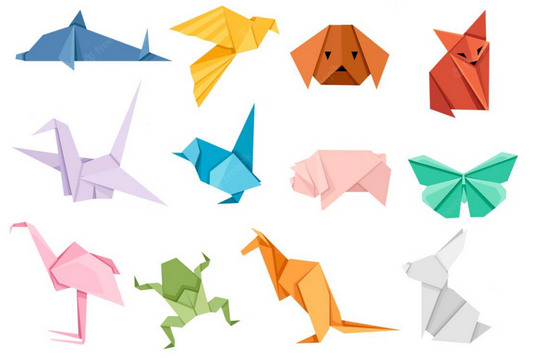
\includegraphics[width=0.5\textwidth]{a.png}
	\end{wrapfigure}
	でんとうてきには
	\begin{itemize}
		\item かみを切らないで、
		\item なにもはらないで、
		\item 四角のかみをつかいます。
	\end{itemize}
\end{frame}
\begin{frame}
	\begin{wrapfigure}{l}{0.5\textwidth}
			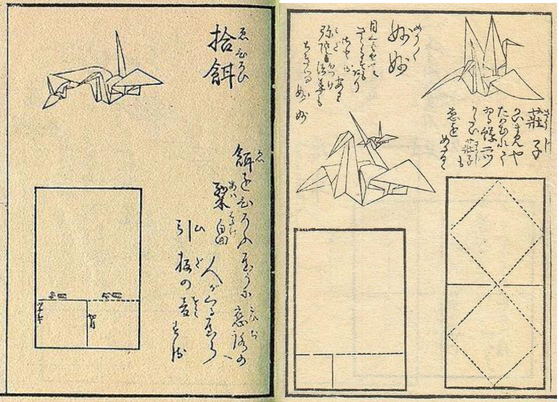
\includegraphics[width=0.5\textwidth]{aa.png}
	\end{wrapfigure}
	むかし。。。
	\begin{itemize}
		\item かみは高かったです、
		\item 折り紙は口頭で
		
		おしえられていました、
		\item 一千七百九十七年:\\「ひでんせんばづる\\おりかた」。
	\end{itemize}
\end{frame}
\begin{frame}
	\begin{wrapfigure}{l}{0.5\textwidth}
			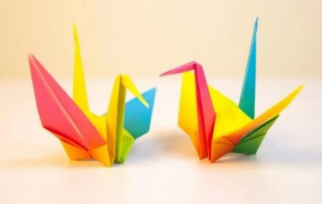
\includegraphics[width=0.5\textwidth]{aaa.png}
	\end{wrapfigure}
    日本で折り紙は
    
    とてもにんきがあります。
    
    つるは
    \begin{itemize}
    	\item けんこう\footnote{Saúde}と
    	\item へいわ\footnote{Paz}と
    	\item しあわせ\footnote{Felicidade}をあらわします
    \end{itemize}
    
    
     
\end{frame}
\begin{frame}

	折り紙デ-は11月11日です。\\
    だいいちじせかいたいせん\footnote{Primeira Guerra Mundial}
    のさいごの日です。
    \center
    
\includegraphics[scale=0.2]{c.jpg}
\end{frame}

\section{ユ-チュ-ブ}
\begin{frame}{ユ-チュ-ブ}
	折り紙はユ-チュ-ブでやさしくおしえられています。
	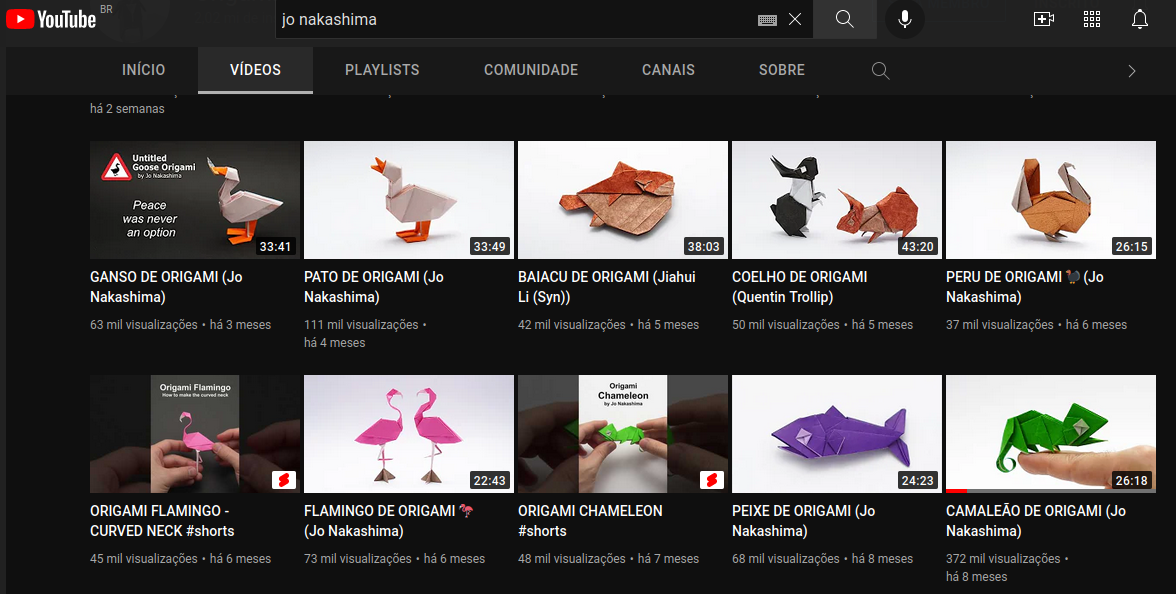
\includegraphics[width=1\textwidth]{b.png}
\end{frame}
\section{折り紙とこうがく}
\begin{frame}{ロボットこうがく\footnote{Robótica}}
		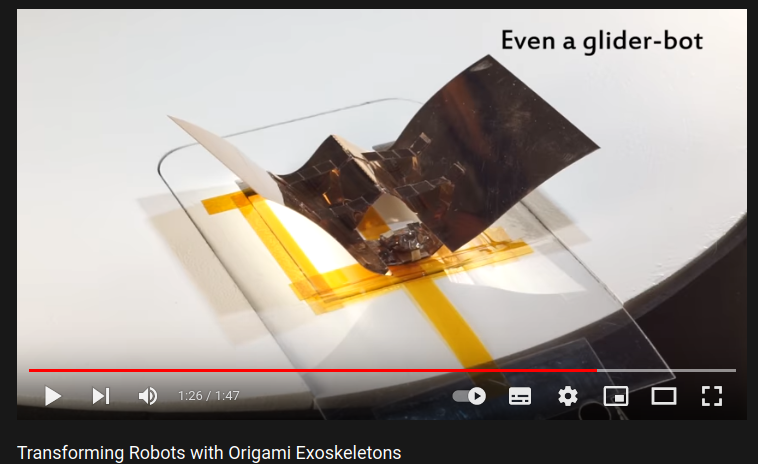
\includegraphics[width=1\textwidth]{bb.png}
	
\end{frame}
\begin{frame}{けんちくがく\footnote{Arquitetura}}
	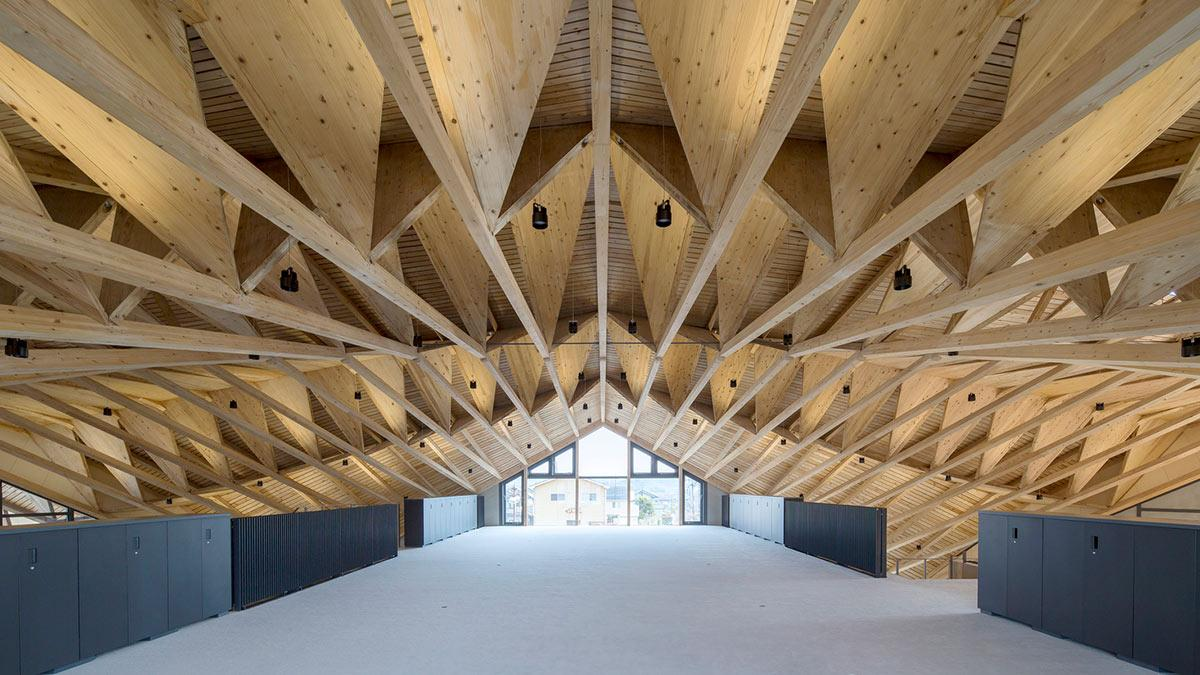
\includegraphics[width=1\textwidth]{b.jpg}
\end{frame}
\begin{frame}{こうくううちゅうこうがく\footnote{Engenharia aeroespacial}}
	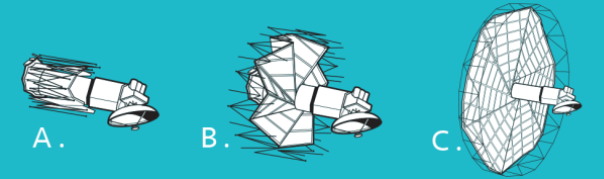
\includegraphics[width=1\textwidth]{c.png}
\end{frame}
\begin{frame}
	\Huge
	\center
	ありがとうございました。
\end{frame}
\end{document}